Zbog pravedne usporedbe, korišteni su modeli koji su trenirani na COCO skupu podataka, a osim YOLO v3, svi modeli su implementirani u sklopu Tensorflow Object Detection API-ja. Budući da u trenutku pisanja Tensorflow Object Detection API ne podržava YOLO, za evaluaciju YOLO v3 je korištena originalna implementacija autora. Modeli su evaluirani na skupovima INRIA People, PeopleArt i Pascal VOC 2012 koristeći samo oznake koje se odnose na osobe. Za usporedbu modela koristili smo srednju preciznost. Srednja preciznost se računa kao omjer broja točnih detekcija i ukupnog broja detekcija. Točna detekcija je ona koja ima omjer presjeka i unije sa stvarnim prozorom oko objekta veći od $0.5$. Ako postoji više detekcija istog objekta, prva se uzima kao točna dok su ostale netočne. Srednje preciznosti detekcije su prikazane u tablici \ref{tablica_preciznosti}. Imena modela u tablici osim samog imena modela sadrže i ime konvolucijske mreže koja se koristi za izlučivanje značajki.

\begin{table}[h]
	\begin{center}
	\begin{tabular}{| c | c | c | c |}
		\hline
		Model & INRIA & PeopleArt & Pascal VOC 2012 \\ \hline
		Faster R-CNN inception v2 & 97.77\% & 57.40\% & 76.10\% \\ \hline
		SSD mobilenet v2 & 87.07\% & 35.39\% & 68.42\% \\ \hline
		SSD inception v2 & 90.87\% & 50.64\% & 71.60\% \\ \hline
		R-FCN ResNet101 & 96.73\% & 48.69\% & 72.72\% \\ \hline
		YOLO v3 & 96.81\% & 66.87\% & 58.43\%  \\ \hline 
	\end{tabular}

	\caption{Tablica prosječnih preciznosti modela za različite skupove podataka.}
	\label{tablica_preciznosti}
	\end{center}
\end{table}

Na skupu INRIA najbolje rezultate postiže Faster R-CNN nakon kojeg slijede R-FCN i YOLO dok su obje inačice SSD modela znatno lošije u detekciji ljudi. Na Pascal VOC 2012, poredak modela po preciznosti je sličan kao i na INRIA skupu osim što YOLO postiže lošije rezultate od svih modela. Međutim, na PeopleArt skupu, YOLO je puno precizniji od ostalih modela.
Općenito, najbolje rezultate algoritmi postižu na INRIA skupu podataka u kojem su ljudi u prvom planu i zauzimaju velik dio slike, a nešto lošije rezultate postižu na skupu Pascal VOC 2012 koji se također sastoji od fotografija, ali se ljudi pojavljuju i u manjim veličinama u odnosu na sliku.
Tipične pogreške Faster R-CNN modela su višestruka detekcija i lažna detekcija. Primjeri pogrešaka su prikazani na slici \ref{faster_greske}.

\begin{figure}[H]
\begin{center}
\subfloat{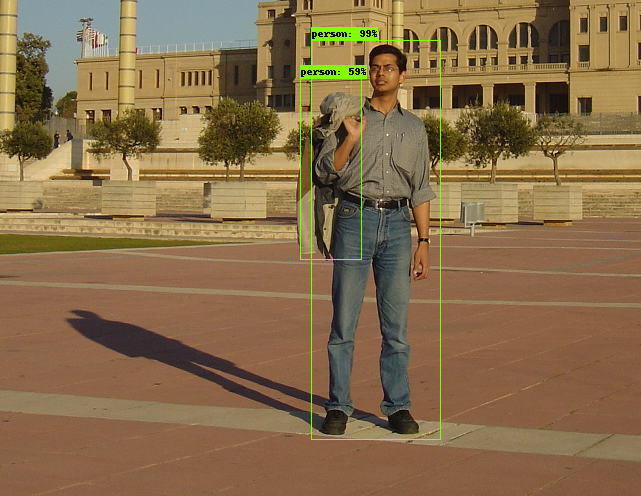
\includegraphics[height = 1.8in]{img/faster_err/crop_000003}} \
\subfloat{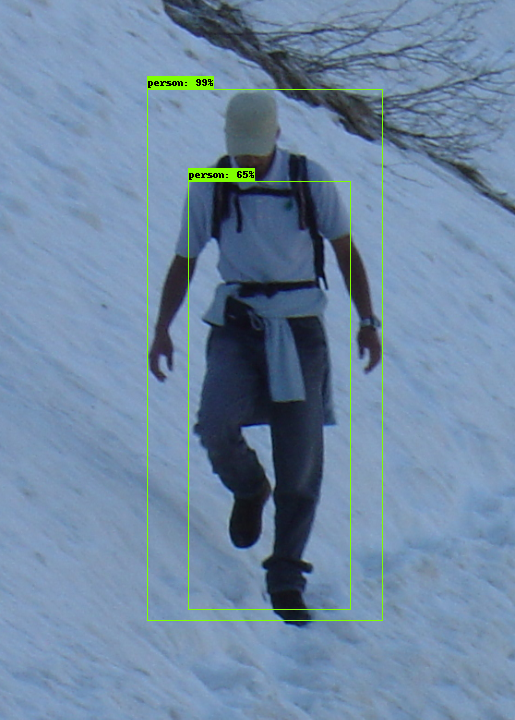
\includegraphics[height = 1.8in]{img/faster_err/crop_000006}} \
\subfloat{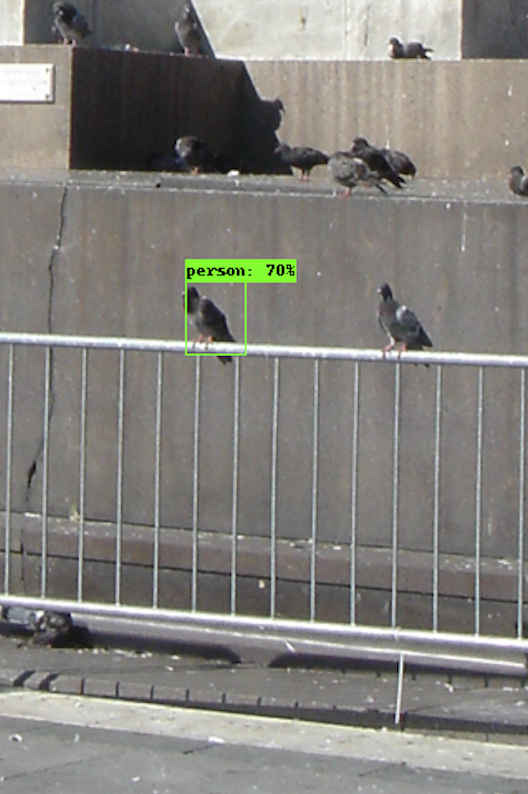
\includegraphics[height = 1.8in]{img/faster_err/golub}}
\caption{Primjeri pogrešaka detekcije Faster R-CNN modelom.}
\label{faster_greske}
\end{center}
\end{figure}
R-FCN, kao i Faster R-CNN, najčešće griješi višestrukim detekcijama, osobito kada se na slici nalazi više ljudi u skupini što je vidljivo u primjerima na slici \ref{rfcn_greske}.

\begin{figure}[H]
\subfloat{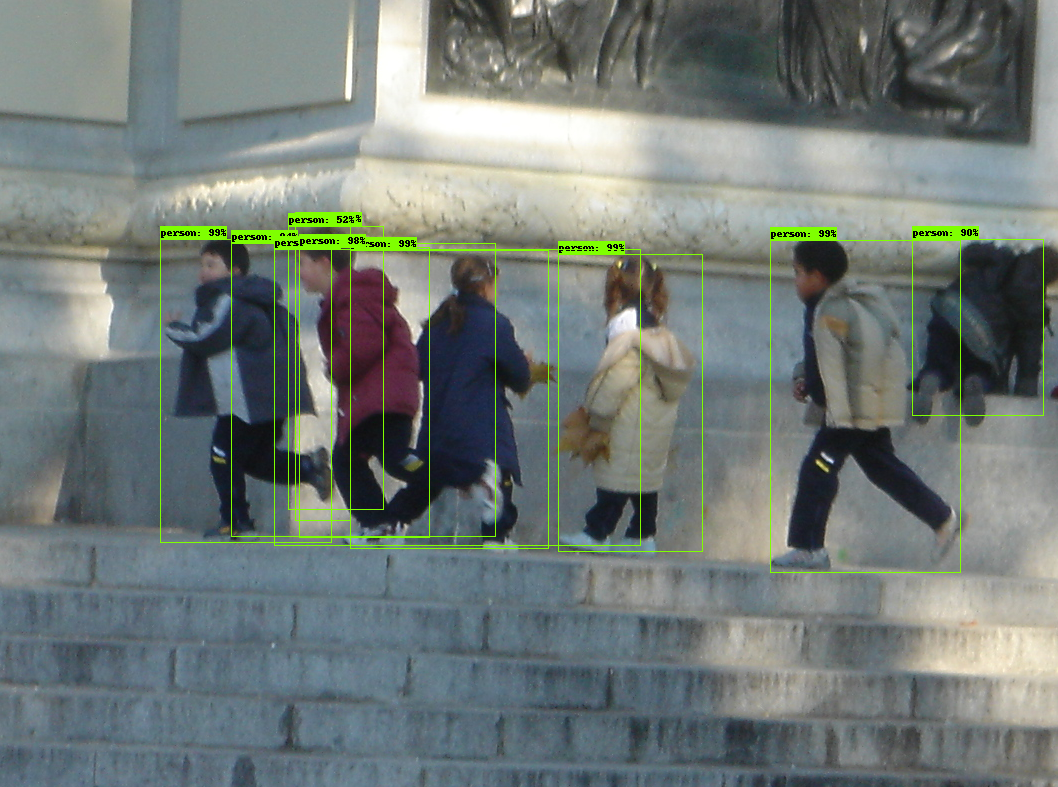
\includegraphics[height = 2.1in]{img/rfcn_err/crop001670}} \
\subfloat{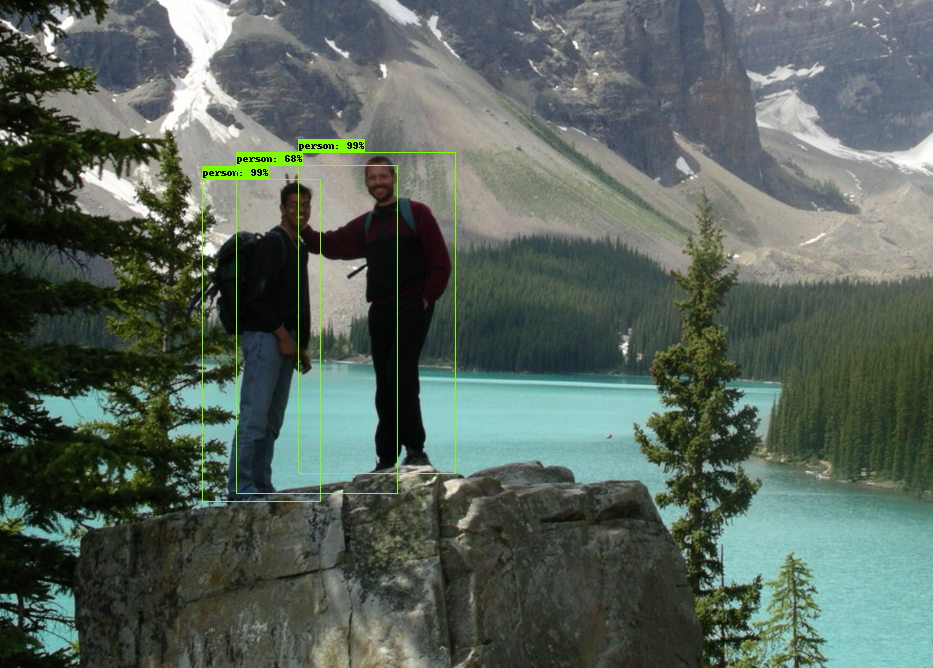
\includegraphics[height = 2.1in]{img/rfcn_err/crop001683}}
\caption{Pogreške višestruke detekcije modela R-FCN.}
\label{rfcn_greske}
\end{figure}

Za razliku od Faster R-CNN-a i R-FCN-a, SSD ima zanemariv broj višestrukih i lažnih detekcija. Najčešće pogreške SSD modela se događaju kada se na slici više osoba nalazi jedna pored druge. U takvim slučajevima model može prepoznati više osoba kao jednu ili prepoznati samo jednu osobu a druge u blizini zanemariti. Osim toga, u nekim slučajevima ne prepoznaje osobe okrenute leđima ili bočno. Na slici \ref{ssd_greske} su prikazani primjeri najčešćih pogrešaka.

\begin{figure}[H]
\subfloat{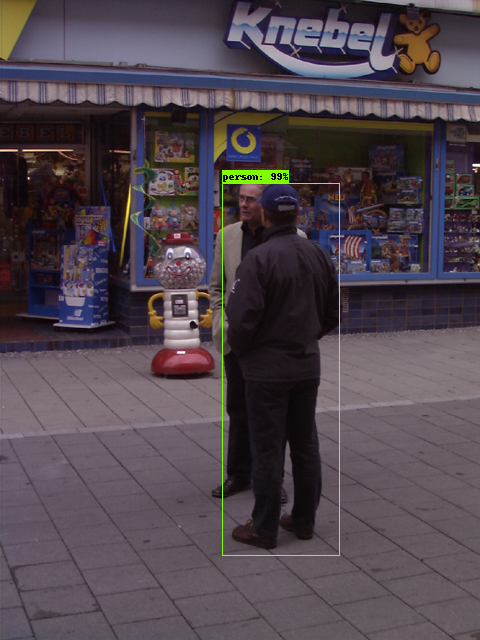
\includegraphics[height = 1.6in]{img/ssd_err/person_087}} \
\subfloat{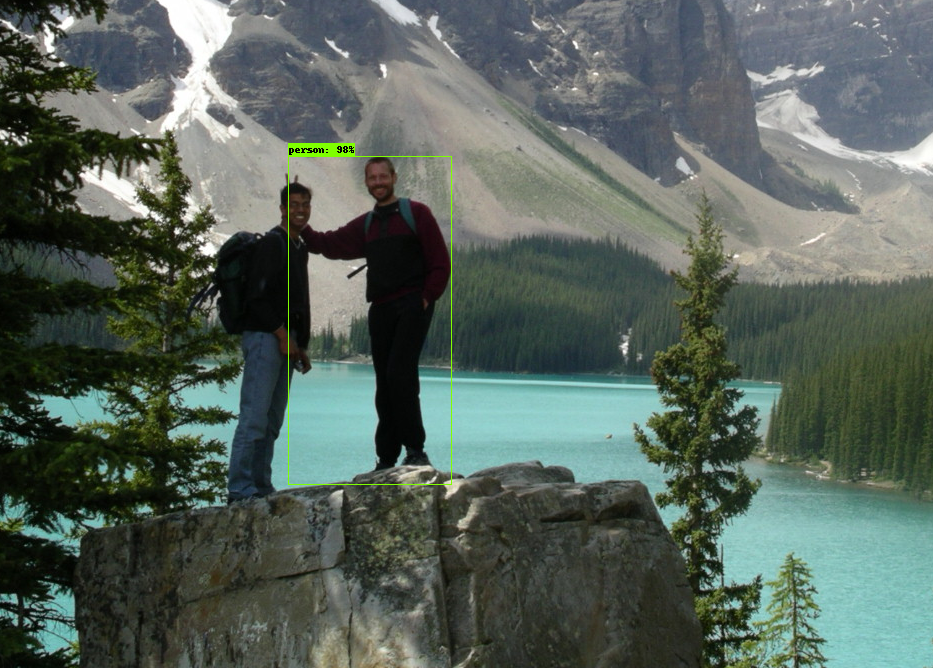
\includegraphics[height = 1.6in]{img/ssd_err/crop001683}} \
\subfloat{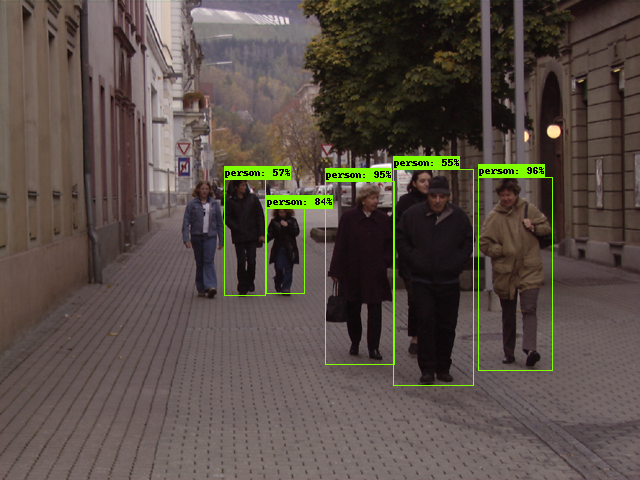
\includegraphics[height = 1.6in]{img/ssd_err/person_191}}
\caption{Primjeri pogrešaka detekcije SSD modelom.}
\label{ssd_greske}
\end{figure}

YOLO ima mali broj lažnih detekcija i u usporedbi s ostalim algoritmima je izuzetno dobar u detekciji ljudi koji su u daljini i relativno mali u odnosu na veličinu slike. Međutim, YOLO najčešće griješi tako da ne prepoznaje ljude koji su bliže kameri i relativno veliki u odnosu na sliku. Primjeri pogrešaka su prikazani na slici \ref{yolo_greske}.

\begin{figure}[H]
\subfloat{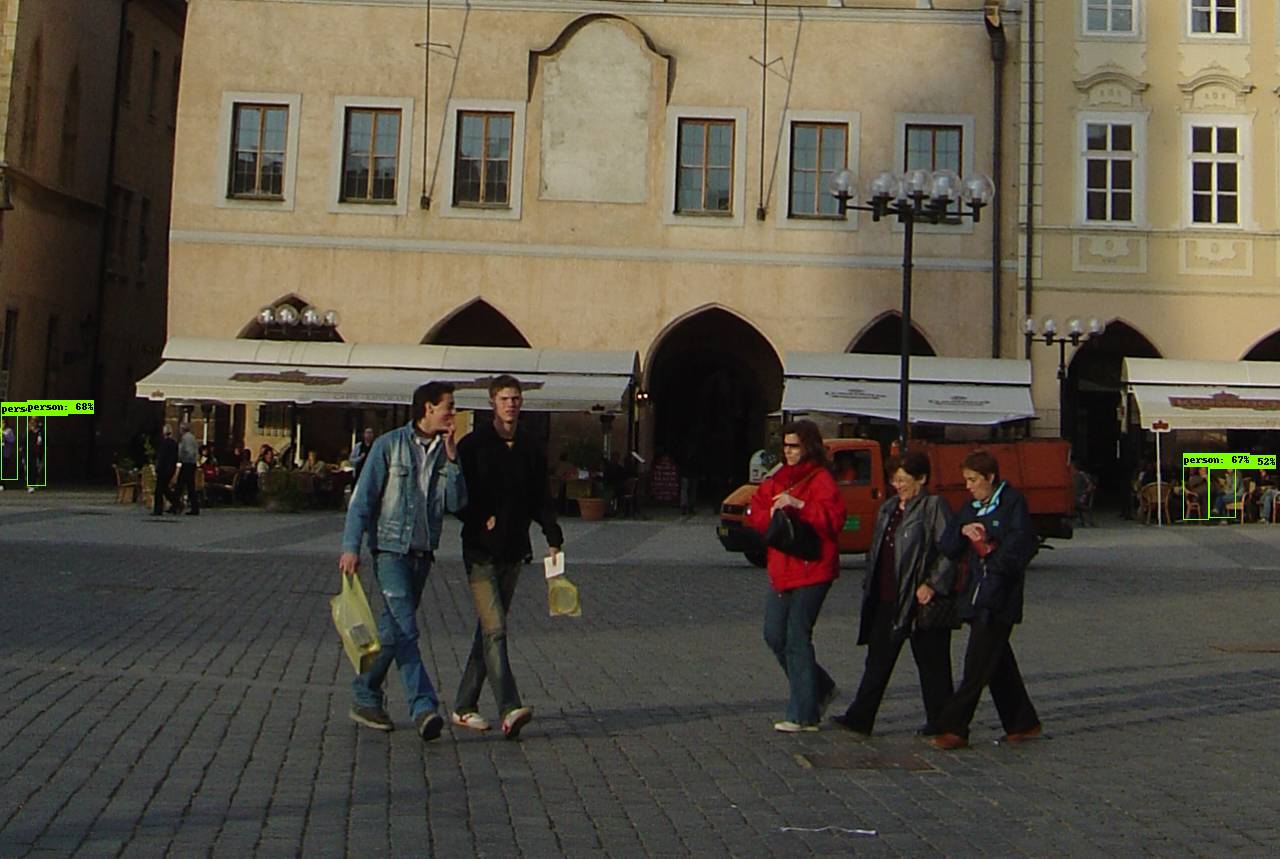
\includegraphics[height = 2in]{img/yolo_err/crop001719}} \
\subfloat{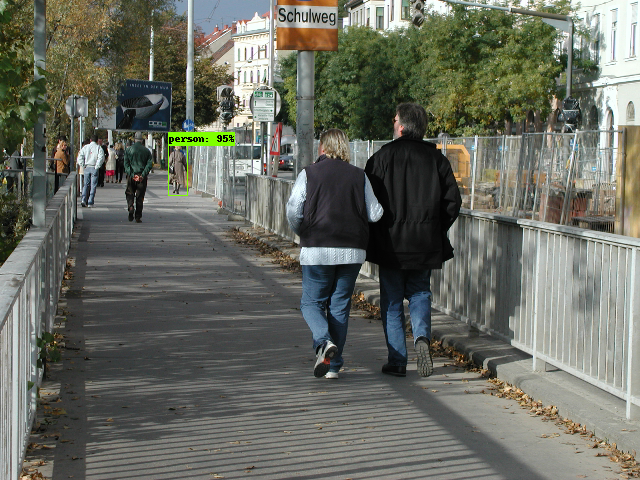
\includegraphics[height = 2in]{img/yolo_err/person_336}}
\caption{Primjeri pogrešaka detekcije YOLO v3 modelom.}
\label{yolo_greske}
\end{figure}


PeopleArt skup podataka je korišten kako bi se provjerilo koliko dobro modeli generaliziraju. Ideja je preuzeta iz \cite{DBLP:journals/corr/RedmonDGF15} gdje autori na istom skupu testiraju YOLO. Iz tablice \ref{tablica_preciznosti} je vidljivo da su preciznosti detekcije svih modela značajno lošije na PeopleArt skupu u odnosu na ostale skupove podataka. Najbolji rezultat postiže YOLO te je za $9.47\%$ bolji od Faster R-CNN koji je na drugom mjestu. SSD s inception v2 mrežom postiže bolje rezultate od R-FCN-a koji je na ostalim skupovima podataka bolji.
Općenito, svi modeli griješe tako da ne detektiraju ljude, posebno ako su ljudi apstraktnije prikazani (Slika \ref{svi_greske}). Faster R-CNN i R-FCN za ljude koje prepoznaju često imaju višestruke detekcije, dok SSD često griješi na slikama sa slabijim kontrastom. Najčešće greške YOLO detektora su prepoznavanje više ljudi kao jednog čovjeka i predviđanje prevelikih prozora za pojedinu osobu.

\begin{figure}[H]
\begin{center}
\subfloat{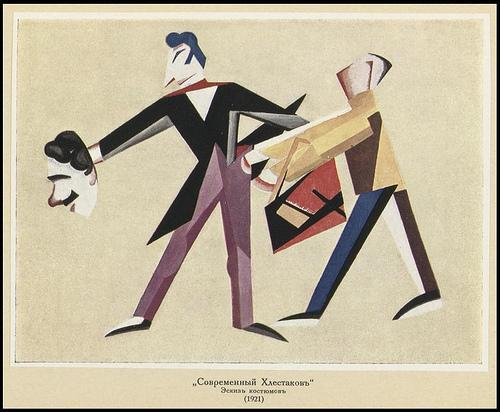
\includegraphics[height = 2in]{img/err_all/aleksandra-ekster_costume-design-for-modern-khlestakov-1921}} \
\subfloat{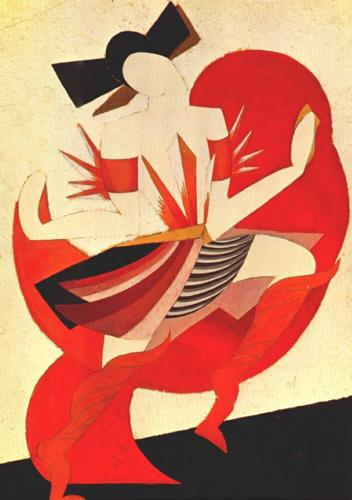
\includegraphics[height = 2in]{img/err_all/aleksandra-ekster_costume-for-romeo-and-juliet-1920}} \
\subfloat{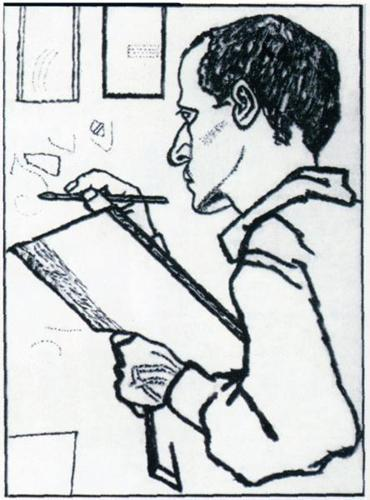
\includegraphics[height = 2in]{img/err_all/pavel-filonov_selfportrait-1925}}
\caption{Primjeri slika na kojima nijedan model ne prepoznaje osobe.}
\label{svi_greske}
\end{center}
\end{figure}

\begin{figure}[H]
\begin{center}
\subfloat{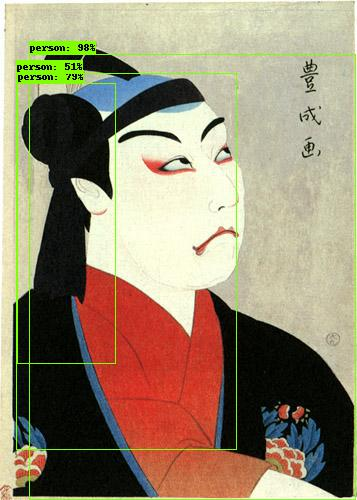
\includegraphics[height = 2in]{img/faster_err/yamamura-toyonari_matsumoto-koshiro-vii-as-sukeroku-1920}} \
\subfloat{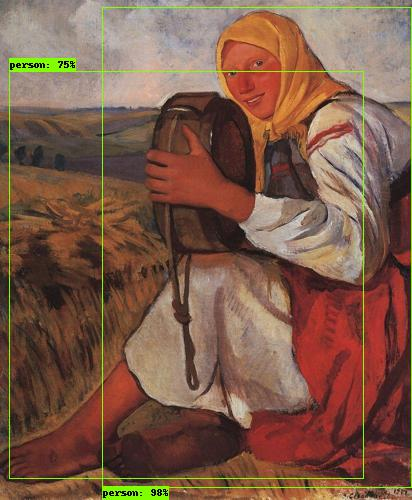
\includegraphics[height = 2in]{img/faster_err/zinaida-serebriakova_peasant-1914}} \
\subfloat{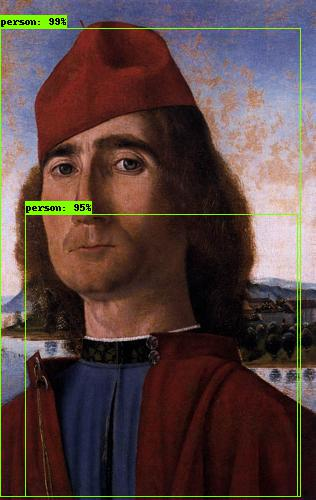
\includegraphics[height = 2in]{img/faster_err/vittore-carpaccio_portrait-of-an-unknown-man-with-red-beret-1493}}
\caption{Primjeri pogrešaka višestruke detekcije Faster R-CNN modelom na PeopleArt skupu podataka.}
\end{center}
\end{figure}

\begin{figure}[H]
\begin{center}
\subfloat{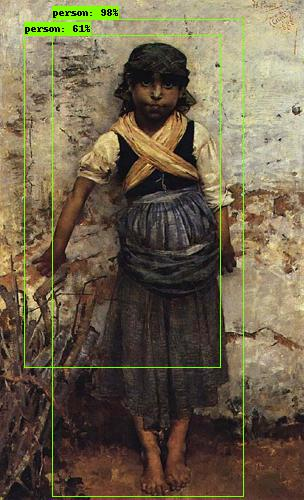
\includegraphics[height = 2in]{img/rfcn_err/henrique-pousao_cansada-1882}} \
\subfloat{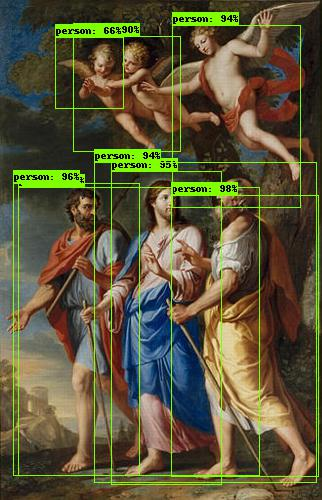
\includegraphics[height = 2in]{img/rfcn_err/jacques-stella_the-pilgrims-of-emmaus}} \
\subfloat{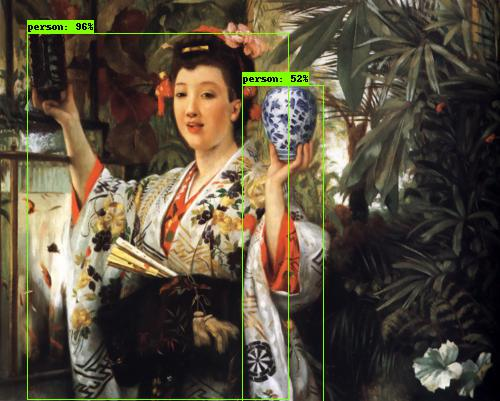
\includegraphics[height = 2in]{img/rfcn_err/james-tissot_the-japanese-vase}}
\caption{Primjeri pogrešaka višestruke detekcije R-FCN modelom na PeopleArt skupu podataka.}
\end{center}
\end{figure}

\begin{figure}[H]
\begin{center}
\subfloat{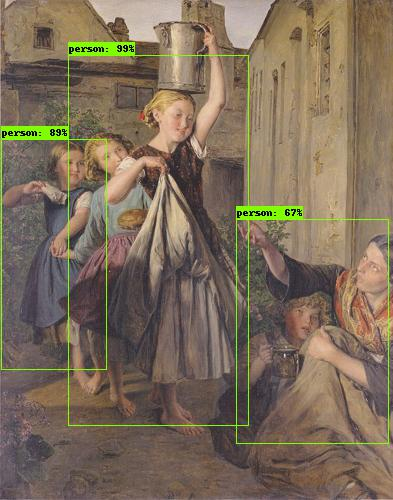
\includegraphics[height = 2in]{img/yolo_err/ferdinand-georg-waldm-ller_charity-1863}} \
\subfloat{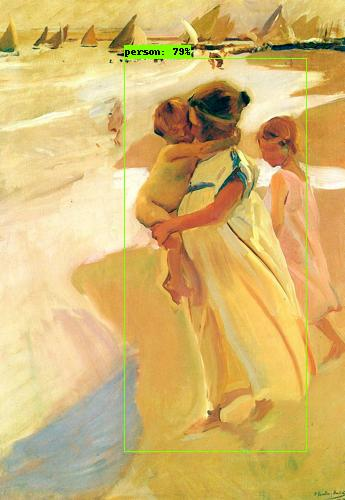
\includegraphics[height = 2in]{img/yolo_err/joaqu-n-sorolla_after-bathing-valencia-1908}} \
\subfloat{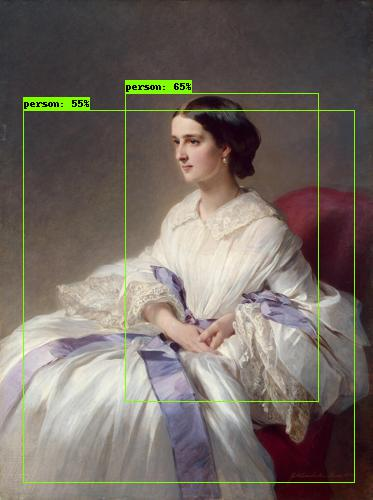
\includegraphics[height = 2in]{img/yolo_err/franz-xaver-winterhalter_portrait-of-countess-olga-shuvalova}}
\caption{Primjeri pogrešaka detekcije YOLO v3 modelom na PeopleArt skupu podataka.}
\end{center}
\end{figure}

Algoritmi su testirani i na slikama visoke rezolucije s nogometne utakmice na kojima se vidi cijeli teren. Budući da slike prikazuju veliki prostor odjednom, igrači su vrlo mali u odnosu na sliku i niti jedan algoritam ne prepoznaje niti jednog igrača. Na slici rezolucije $3260 \times 570$ visine igrača se kreću u rasponu od 20 do 60 piksela, ovisno o udaljenosti od kamere. Međutim, ako se slika podijeli na manje dijelove ($326 \times 285$) i ako se za svaki dio posebno napravi predikcija te se rezultati na kraju spoje u jednu sliku, dobivaju se zanimljivi rezultati. Detekcije različitih algoritama za sliku koja je prilikom detekcije podijeljena na mrežu $2 \times 10$ su prikazane na slikama \ref{nogomet_ssd_mobilenet}, \ref{nogomet_ssd_inception}, \ref{nogomet_rfcn}, \ref{nogomet_faster} i \ref{nogomet_yolo}. Zbog velikih dimenzija, slike su prikazane u dva dijela (lijevi i desni dio terena).

\begin{figure}[h]
\begin{center}
\subfloat{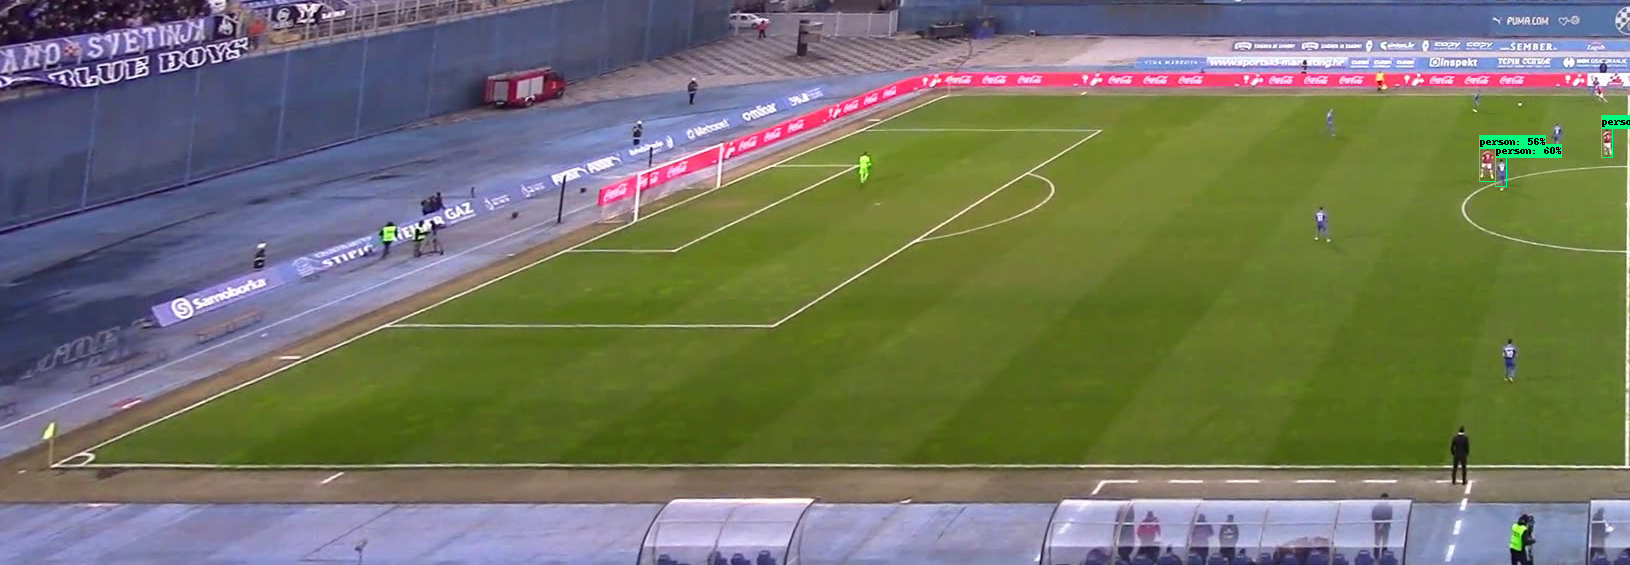
\includegraphics[scale=0.25]{img/inference_by_parts/snapshot_ssd_mobilenet_l}} \\
\subfloat{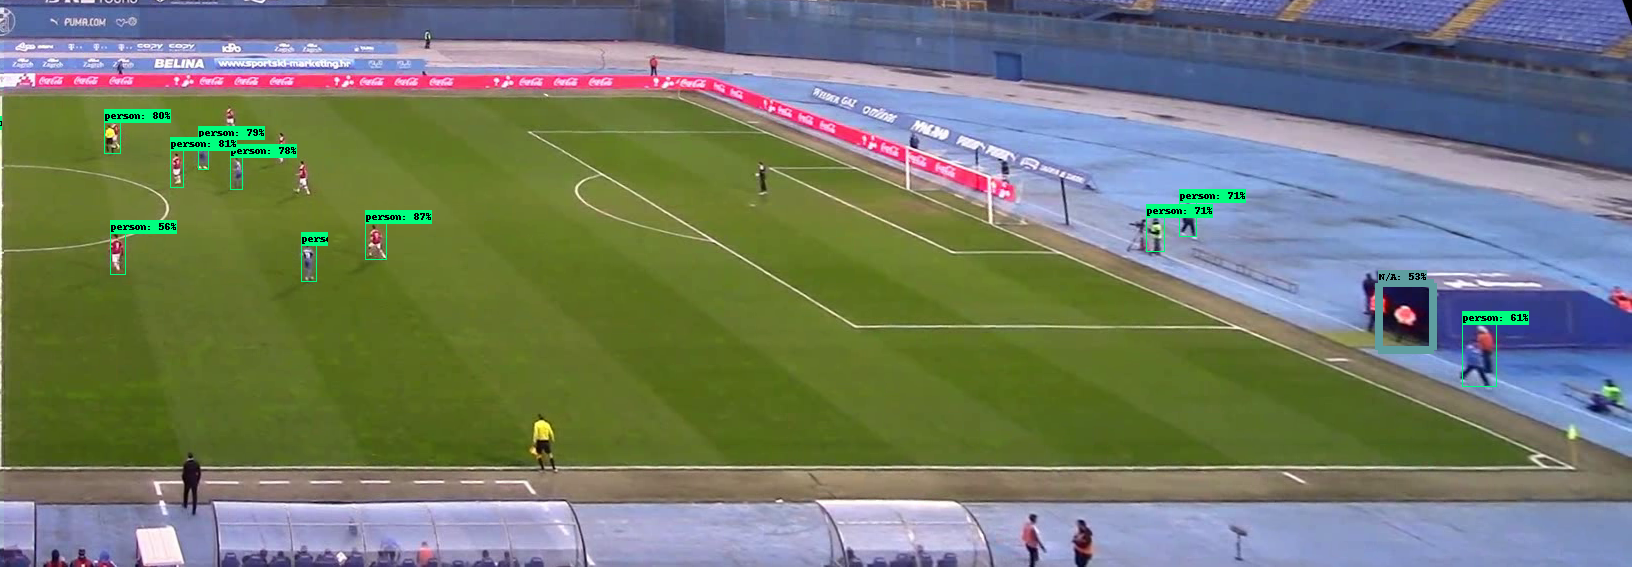
\includegraphics[scale=0.25]{img/inference_by_parts/snapshot_ssd_mobilenet_r}}
\caption{Detekcija igrača, sudaca i ostalih osoba na nogometnoj utakmici modelom SSD mobilenet v2.}
\label{nogomet_ssd_mobilenet}
\end{center}
\end{figure}

\begin{figure}[h]
\begin{center}
\subfloat{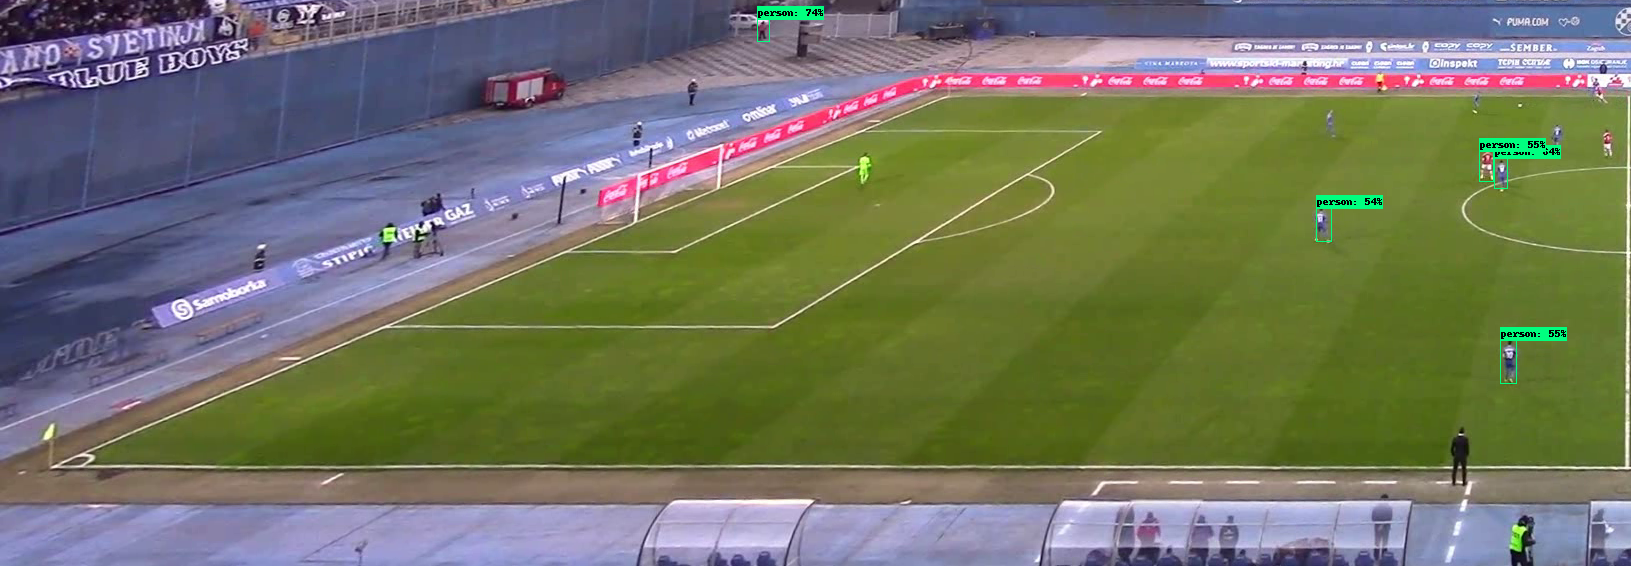
\includegraphics[scale=0.25]{img/inference_by_parts/snapshot_ssd_inception_l}} \\
\subfloat{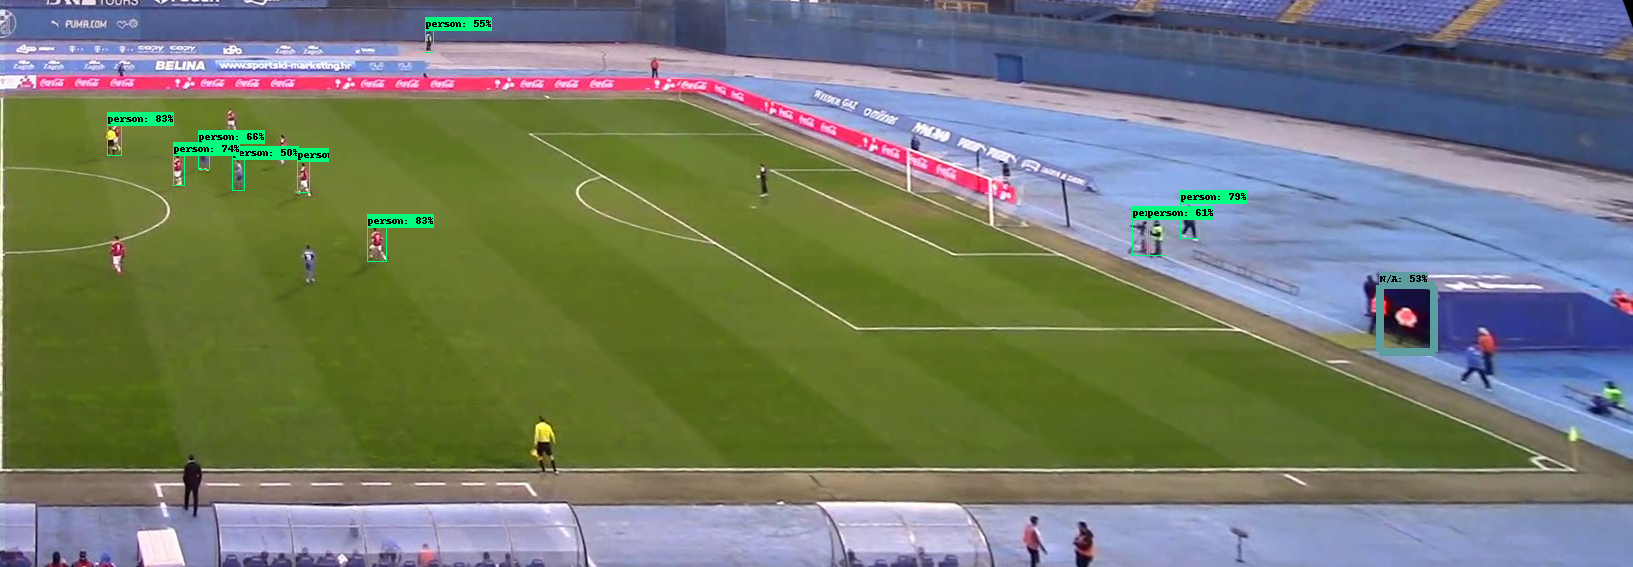
\includegraphics[scale=0.25]{img/inference_by_parts/snapshot_ssd_inception_r}}
\caption{Detekcija igrača, sudaca i ostalih osoba na nogometnoj utakmici modelom SSD inception v2.}
\label{nogomet_ssd_inception}
\end{center}
\end{figure}

\begin{figure}[h]
\begin{center}
\subfloat{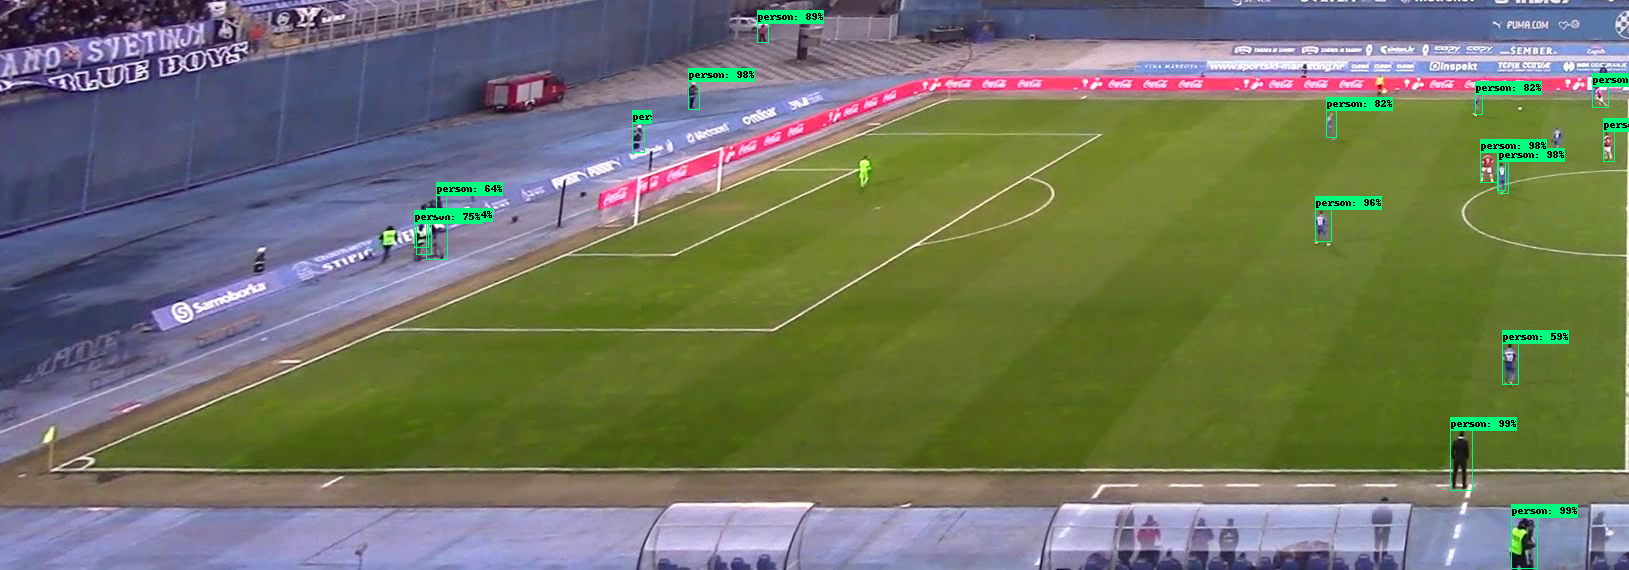
\includegraphics[scale=0.25]{img/inference_by_parts/snapshot_rfcn_l}} \\
\subfloat{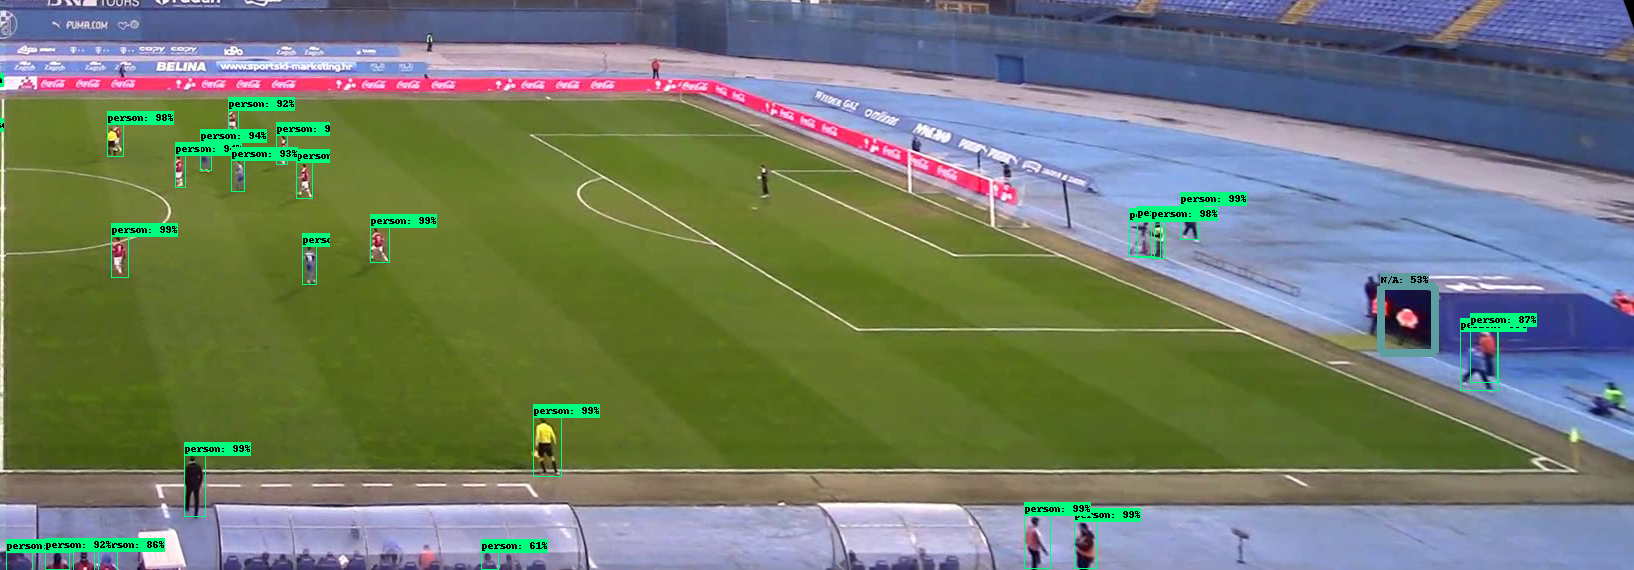
\includegraphics[scale=0.25]{img/inference_by_parts/snapshot_rfcn_r}}
\caption{Detekcija igrača, sudaca i ostalih osoba na nogometnoj utakmici modelom R-FCN.}
\label{nogomet_rfcn}
\end{center}
\end{figure}

\begin{figure}[h]
\begin{center}
\subfloat{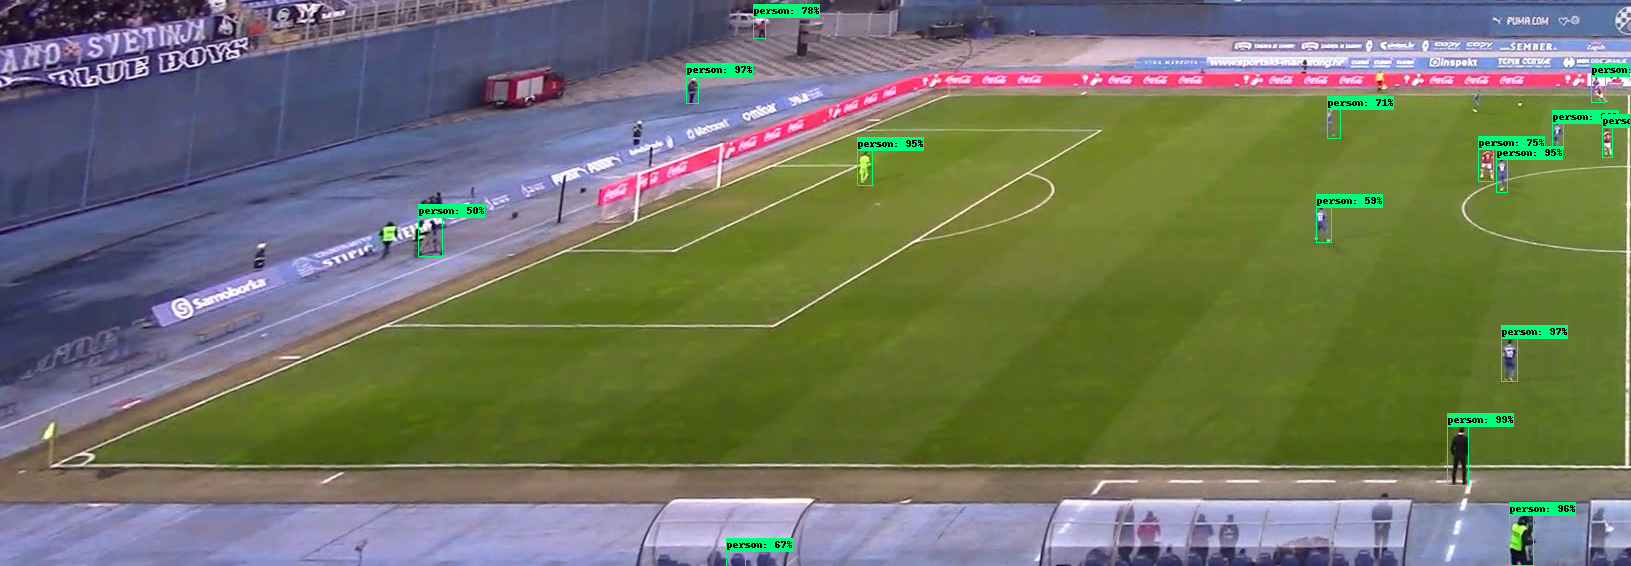
\includegraphics[scale=0.25]{img/inference_by_parts/snapshot_faster_l}} \\
\subfloat{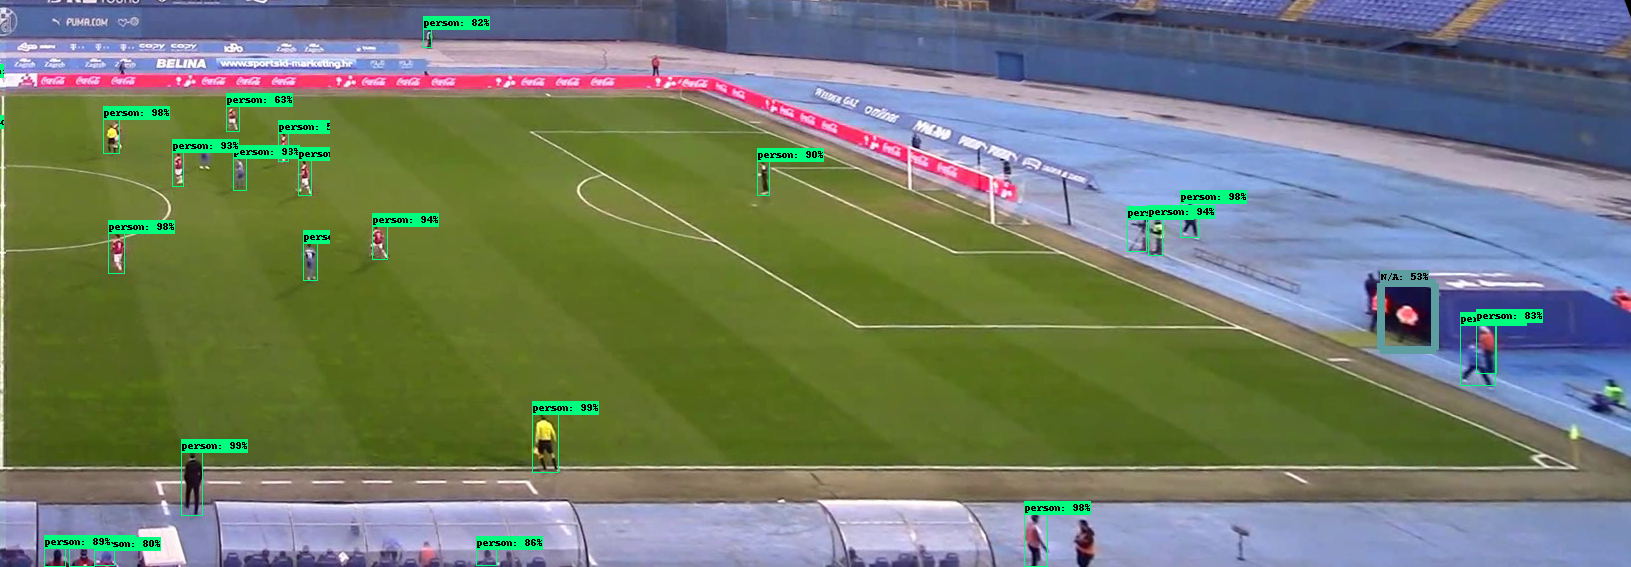
\includegraphics[scale=0.25]{img/inference_by_parts/snapshot_faster_r}}
\caption{Detekcija igrača, sudaca i ostalih osoba na nogometnoj utakmici modelom Faster R-CNN.}
\label{nogomet_faster}
\end{center}
\end{figure}

\begin{figure}[h]
\begin{center}
\subfloat{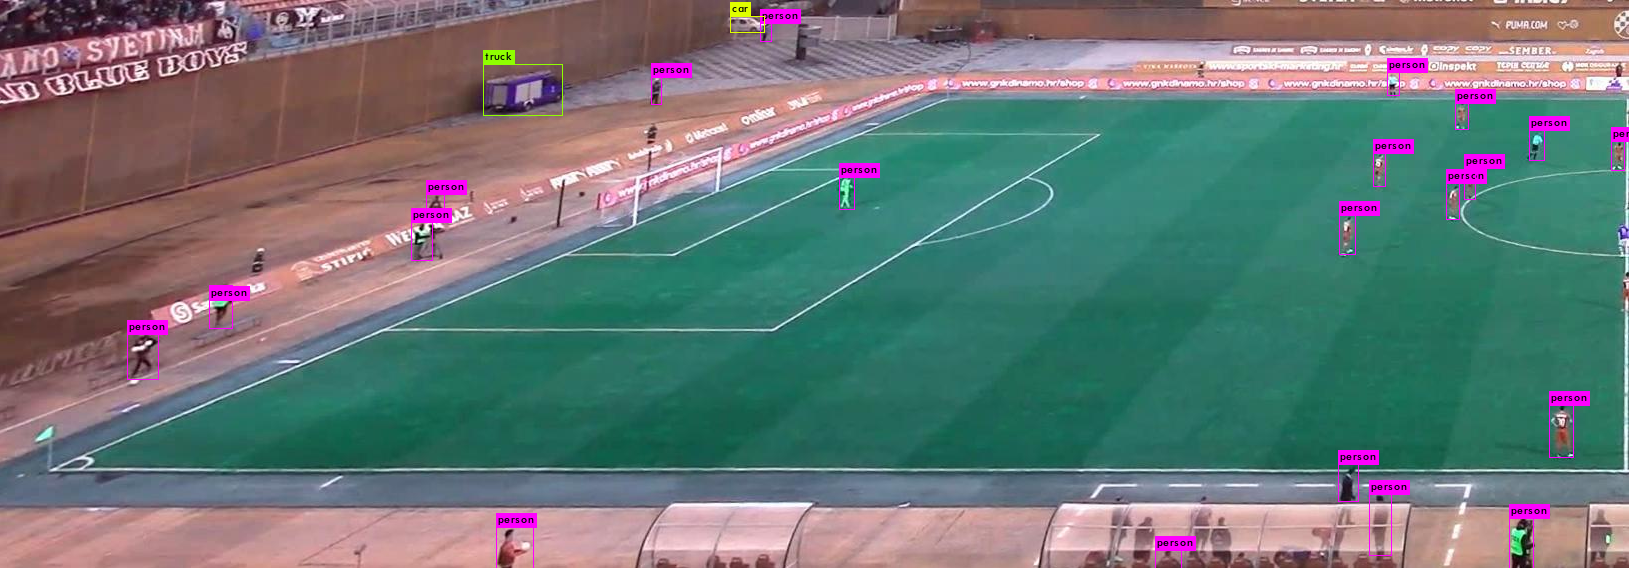
\includegraphics[scale=0.25]{img/inference_by_parts/snapshot_yolo_l}} \\
\subfloat{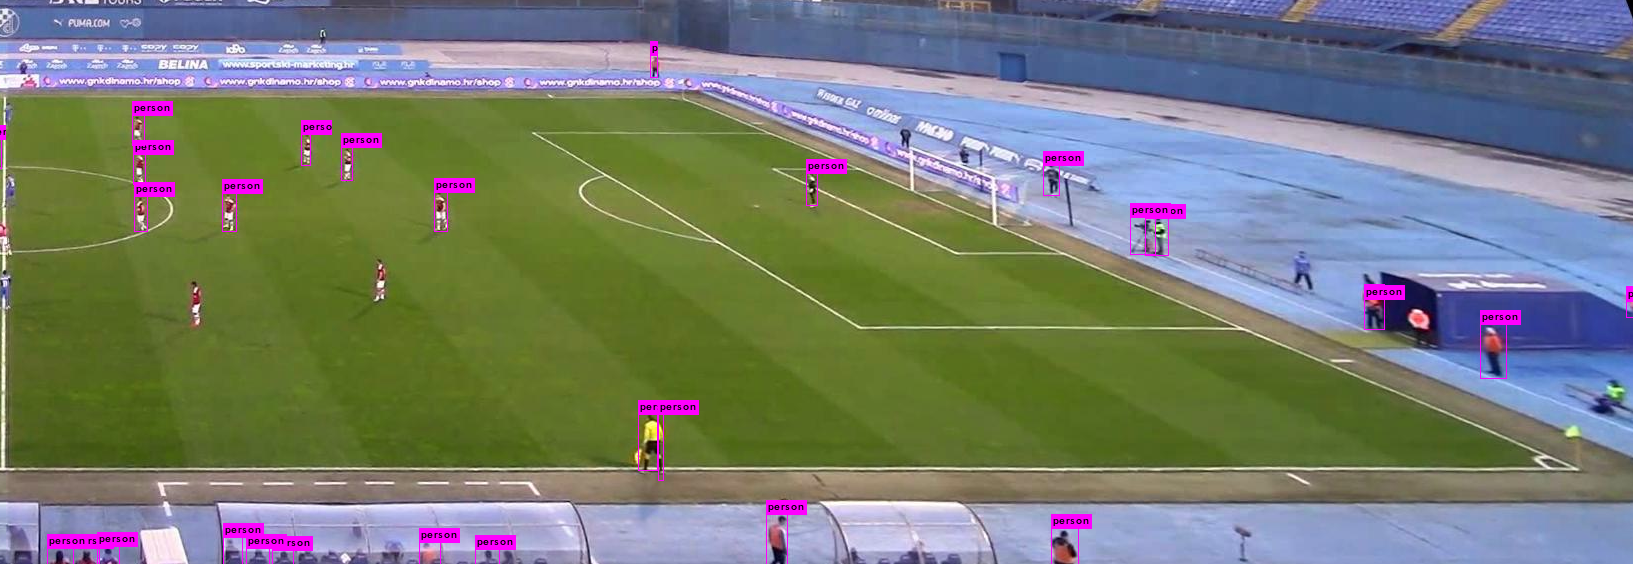
\includegraphics[scale=0.25]{img/inference_by_parts/snapshot_yolo_r}}
\caption{Detekcija igrača, sudaca i ostalih osoba na nogometnoj utakmici modelom YOLO v3.}
\label{nogomet_yolo}
\end{center}
\end{figure}